\onecolumn{}
\begin{figure}
\begin{adjustbox}{minipage={\linewidth},frame}
\vspace{2.5mm}
\centering

\def\picdir{readmitted30d/}
\def\picroc{readmitted30d_ROC.pdf}
\def\piccal{readmitted30d_cal.pdf}
\def\picbar{readmitted30d_SHAP_summary_bar.pdf}
\def\picsum{readmitted30d_SHAP_summary.pdf}
\def\picfpone{readmitted30d_10_SHAP_Pt_17807.png}
\def\picfptwo{readmitted30d_280_SHAP_Pt_11558.png}
\def\picfpthr{readmitted30d_10_SHAP_Pt_18181.png}

\begin{subfigure}[t]{.45\linewidth}
    \centering
    \captionsetup[subfigure]{}
    \caption[t]{Receiver operator characteristic curve.}\label{fig:roc30d}
    % 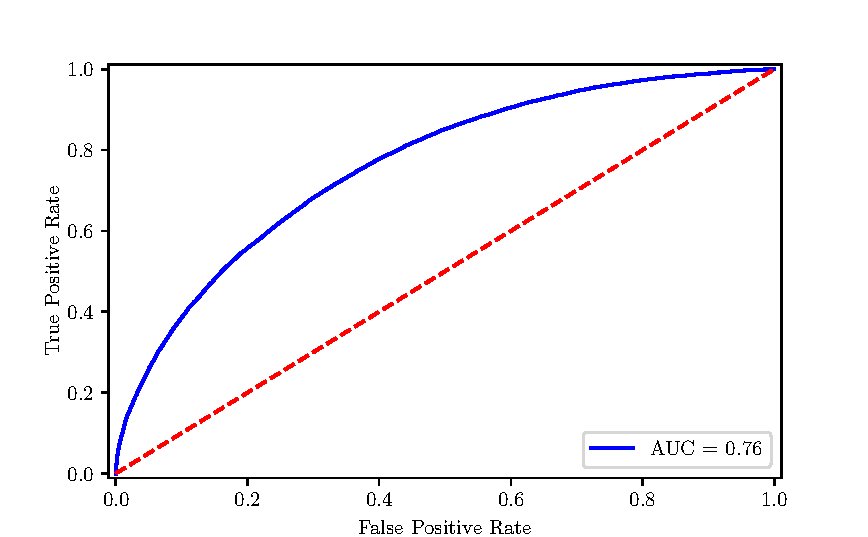
\includegraphics[width=\linewidth,height=.2\textheight,keepaspectratio]{readmitted30d/readmitted30d_ROC.pdf}
    \includegraphics[width=\linewidth,height=.2\textheight,keepaspectratio]{\picdir\picroc}
    % \input{test2.pgf} %% pgf not working for some reason
\end{subfigure}
\begin{subfigure}[t]{.45\linewidth}
    \centering
    \captionsetup[subfigure]{}
    \caption{Calibration curve.}\label{fig:cal30d}
    \includegraphics[width=\linewidth,height=.2\textheight,keepaspectratio]{\picdir\piccal}
    \vspace{2.5mm}
\end{subfigure}

\begin{subfigure}[t]{.45\linewidth}
    \vspace{2.5mm}
    \centering
    \captionsetup[subfigure]{}
    \caption{Bar summary of most impactful features.}\label{fig:shapsumbar30d}
    \includegraphics[width=\linewidth,height=.40\textheight,keepaspectratio]{\picdir\picbar}
    % \vspace{2.5mm}
\end{subfigure}
\begin{subfigure}[t]{.45\linewidth}
    \vspace{2.5mm}
    \centering
    \captionsetup[subfigure]{}
    \caption{Summary of most impactful features.}\label{fig:shapsum30d}
    \vspace{-2.3mm}
    \includegraphics[width=\linewidth,height=.38\textheight,keepaspectratio]{\picdir\picsum}
    \vspace{2.0mm}
\end{subfigure}
\textsf{Individualized predictions with interpretation.}
\vspace{-2.5mm}
\begin{subfigure}[t]{0.1\textwidth}
    \caption{}\label{fig:shapforce30d1}
    \end{subfigure}%
    \begin{minipage}[c]{0.9\textwidth}
    \includegraphics[width=\linewidth,keepaspectratio]{\picdir\picfpone}
    \vspace{-2.5mm}
\end{minipage}
\begin{subfigure}[t]{0.1\textwidth}
    \caption{}\label{fig:shapforce30d2}
    \end{subfigure}%
    \begin{minipage}[c]{0.9\textwidth}
    \includegraphics[width=\linewidth,keepaspectratio]{\picdir\picfptwo}
    \vspace{-3.5mm}
\end{minipage}
\vspace{-4.5mm}
\begin{subfigure}[t]{0.1\textwidth}
    \caption{}\label{fig:shapforce30d3}
    \end{subfigure}%
    \begin{minipage}[c]{0.9\textwidth}
    \includegraphics[width=\linewidth,keepaspectratio]{\picdir\picfpthr}
    \vspace{-2.5mm}
\end{minipage}
\vspace{-2.5mm}

\caption{\textbf{30-day Readmission.} \\
Model performance curves are shown for binary classification (Panel~\ref{fig:roc30d}) and probability calibration (Panel~\ref{fig:cal30d}).
Panels~\ref{fig:shapsumbar30d} and~\ref{fig:shapsum30d} show the most impactful features on prediction, along with the impact of high or low values for numeric features.
Panels~\ref{fig:shapforce30d1}--\ref{fig:shapforce30d3} show the composition of invididualized predictions for three patients. 
}\label{fig:30dreadmission}
\end{adjustbox}
\end{figure}